\section{Results}\label{sec:Results}
During our experimentation with the agent we attempted using multiple different configurations for the agent and the environment.
In this section we will focus on a few significant iterations of the agent and environment that were used during the course of the project.
It will showcase the progress of our agent and inform about different decisions made to improve the agents performance.
We used the average IoU of the agent during training and the mean average precision of the agent on a test data set to evaluate agent performance during the experimentation.


\subsection{Results closest to Paper}
Our training setup for the first agent was following the paper\cite{caicedo2015active} without any modification to the suggested formula from our side.
This setup resulted in an agent which, while being able to focus on the relevant parts of the image, was not able to pull the trigger.
We think this was due to it being able to generate more reward just by hovering around the target bounding box instead of pulling the trigger, which would end the episode and consequentially stop the agent from acquiring any further reward.

\subsection{Experiment 1}
After observing the first trained agent we decided to implement a way of penalizing the agent for long episode duration.
This was done by applying a negative reward for each step taken which would in turn force the agent to end episodes earlier if he was to receive any positive reward.
Using this configuration the agent managed to focus on the correct part of the image and also managed to pull the trigger.
The resulting agent was the first to consistently finish the episodes thus achieving an average IoU of around $0.35$ in a relatively short training run, with our target IoU being $0.6$ during our testing.

\begin{figure}[h!]
    \centering
    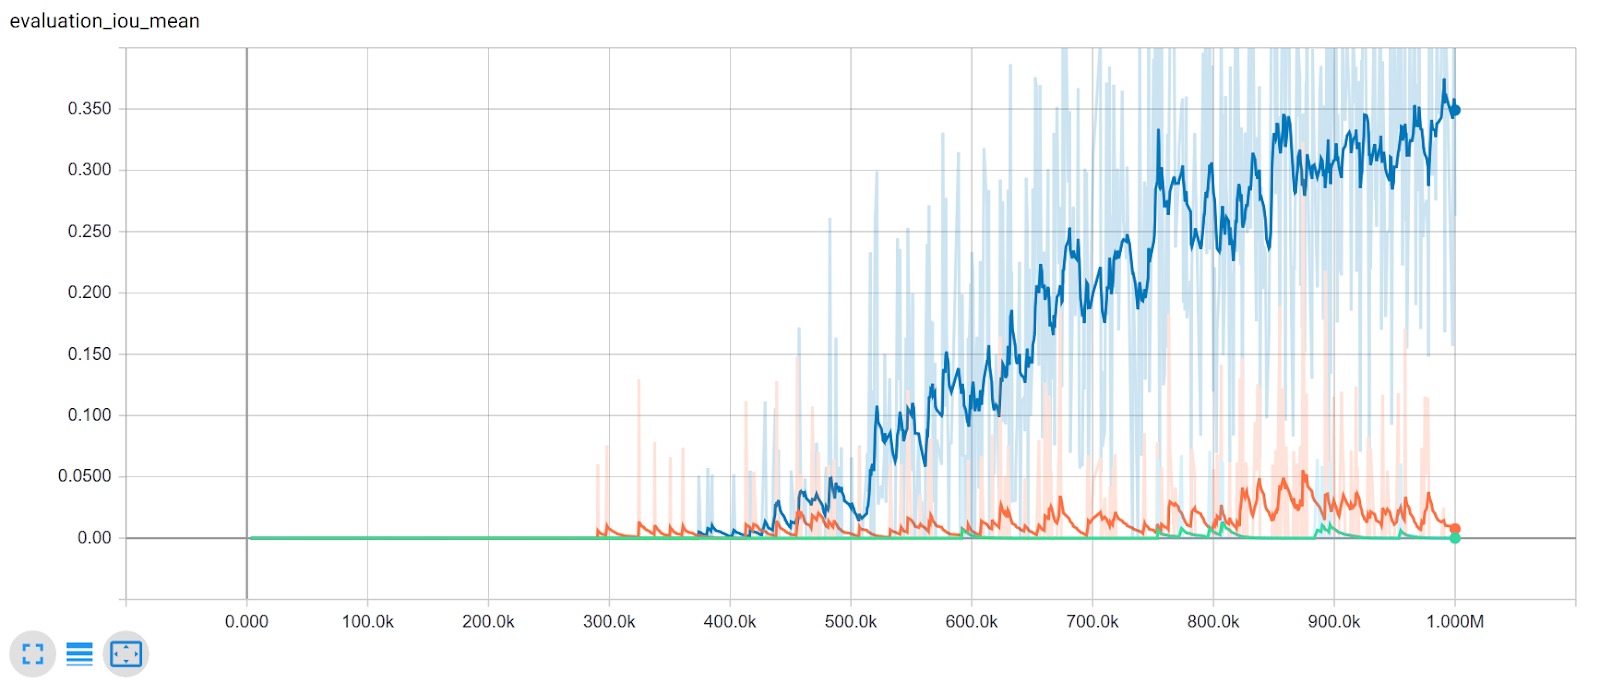
\includegraphics[width=0.7\textwidth]{figures/penalty_results.png}
    \caption{Results from the first Experiment}
\end{figure}

\subsection{Experiment 2}
During our meetings a performance discussion prompted switching the feature extractor from VGG16\cite{VGG16} to ResNet\cite{ResNet} because of ResNet's better applicability in object detection.
The feature extractor switch resulted in a pretty noticeable performance spike in comparison to the old agent.
We achieved an average IoU of $0.64$ with the same target IoU of $0.6$ as in the previous experiment and also managing a mean average precision of $92.74$ percent on our test set generated by the \textit{dataset-generator} described in \ref{sec:dataset-generator}. 

At this point it should be noted, that the average IoU is very unlikely to be substantially higher than the target IoU even with perfect precision. This is the case because under the reward scheme we used the agent has no incentive to strive for an IoU that is higher than the target, the reward will be the same. This means that to achieve an mean IoU significantly higher than the 0.64 achieved is this experiment a higher target IoU would be required.